Posteriormente, con la finalidad de abstraer todos estos modelos matemáticos, y
cálculos, se implementan los sistemas de NN, haciendo uso de distintas
herramientas de libre acceso. tales como sklearn(para ajuste de datos y
creación de modelos basicos de NN.),
seaborn(para visualización de los datos), matplotlib ( visualización de datos),
tensorflow(para realizar modelado de datos con redes neuronales un tanto mas
complejas), Numpy(para trabajar con álgebra lineal.), Pandas(parecido a excel,
tiene como objetivo principal el manejo de datos en python, crear, eliminar,
formatear, limpiar datos perdidos.)

En la sección presente se establecen pequeños bloques de código, y sus respectivas
descripciones.

En el bloque \ref{encabezado1}, muestro como se declaran las librerías a
utilizar, todas de código abierto. 

\begin{lstlisting}[language=Python, caption=Librerías empleados durante el
proceso, label={encabezado1}]
import pandas as pd 
import matplotlib 
import matplotlib.pyplot as plt
import numpy as np
import seaborn as sns
%matplotlib inline
import matplotlib.pyplot as plt
import seaborn as sns
import hvplot.pandas
\end{lstlisting}
Para leer los datos en este casa estamos haciendo uso de las funciones de
panadas 'read\_csv',  dado que el formato en el que tenemos los datos es .csv. 
\begin{lstlisting}[language=Python, caption=Carga de los datos]
df = pd.read_csv("Datos_Enero-Dic2020_estacionUAS_M30min.csv")
df.describe()
\end{lstlisting}
Función para mostrar el formato de los datos.
\begin{lstlisting}[language=Python, caption=Muestra de los datos]
df.head()
\end{lstlisting}
Posterior la salida de la ejecución seria la siguiente
\begin{table}[H]
    \centering
    \begin{tabular}{p{2cm}p{2cm}p{2cm}p{2cm}p{2cm}p{2cm}}\hline
        Temperatura Externa &	Humedad Externa &	Velocidad del viento&
        Radiación Solar&	UV Index & Fecha\\\hline
        20200101 &	17.955& 84.574&	0.887&	48.957&	    0.389\\
        20200102&	17.254&	80.438&	2.800&	189.542&	1.054\\
        20200103&	17.758&	77.812&	3.069&	194.875&	1.021\\
        20200104&	18.798&	72.750&	3.700&	202.354&	1.069\\
        20200105&	20.312&	67.688&	3.267&	201.458&	1.121\\
        \hline
    \end{tabular}
    \caption{Formato de los datos}
    \label{formato de la data}
\end{table}

Para realizar un ajuste del los datos estamos haciendo uso de sklearn, donde se
encuentra una función llamada train\_test\_split, para separar los datos en dos
4 conjuntos diferentes, X\_train que representa el set de entrenamiento de
entrada, y Y\_train que seria las salidas para cada entrada(X\_train), y el set
de pruebas o validación X\_test, y\_test empleado para la comprobación del
modelo y efectos de entrenamiento.


Para realizar esta ajuste, es necesario crear sub-arreglos empleado funciones
propias de pandas, donde se seleccionaran las columnas deseadas, este se
realiza en dos ocasiones para seleccionar la salida definida como y, y la
entrada definida como X.

\begin{lstlisting}[language=Python, caption=Ajuste de los datos]
from sklearn.model_selection import train_test_split
X = fecha[['Humedad Externa', 'Velocidad del viento', 'Radiacion Solar']]
y = fecha['Temperatura Externa']

X_train, X_test, y_train, y_test = train_test_split(X, y, test_size=0.3, random_state=42)
print("\n Arreglo Entrenamiento: Entradas: ",X_train.shape, 
      '\n',"Arreglo Pruebas: Entradas: ",X_test.shape,
      '\n',"Arreglo Entrenamiento: Salidas: ", y_train.shape,
      '\n',"Arreglo Preubas: Salidas: ", y_test.shape, '\n')
\end{lstlisting}
Para modelar con redes neuronales estamos haciendo uso de librerías que
abstraen la complejidad de las operaciones descritas en seccion anterior. 

Como primera instancia se hace uso de tensorflow, keras. como herramientas
principales, en ellas existen distintas funciones, y objetos  mismos con los
que se modelara la estructura de la red neuronal.  

\begin{lstlisting}[language=Python, caption=Librerias empleadas para modelado de NN]
from tensorflow.keras.models import Sequential
from tensorflow.keras.layers import Input, Dense, Activation, Dropout
from tensorflow.keras.optimizers import Adam
\end{lstlisting}


Para el modelado se utiliza el bloque de código \ref{modeladotensorflow}, el
modelo esta compuesto por múltiples capas densas, 2, 128, 32, 1, buscando crear
un modelo de NN que describa el comportamiento de una variable en función de
otras.

En este  caso estamos usando como optimizador Adam, y métrica de error = error
cuadrático medio. 

\begin{lstlisting}[language=Python, caption=Código prinipal, label={modeladotensorflow}]
# 70% datos para entrenamiento, de mi dataset(datos Crudos)
## X = Matriz entrada (TA, DP) = (HR)
X_train = np.array(X_train)
## y = Salida (HR)
y_train = np.array(y_train)

# 30% datos para validacion, de mi dataset(datos Crudos)
## X = Matriz entrada (TA, DP)
X_test = np.array(X_test)
## y = Salida (HR)
y_test = np.array(y_test)


model2 = Sequential()
model2.add(Dense(X_train.shape[1], activation='relu'))
model2.add(Dense(128, activation='relu'))
model2.add(Dropout(0.2))
model2.add(Dense(32, activation='relu'))
model2.add(Dense(1))

model2.compile(optimizer=Adam(0.0001), loss='mse')

r = model2.fit(X_train, y_train,
              validation_data=(X_test,y_test),
              batch_size=16,
              epochs=800)
model2.summary()
\end{lstlisting}
Para declarar la estructura del modelo se esta usando la clase sequential(),
dentro de ella se comienzan a agregar las capas en este casa todas
completamente interconectadas(dense), utilizando algunas capas de corrección
dropout().
\begin{lstlisting}[language=Python, caption=Declaración de la estructura del modelo]
model2 = Sequential()
model2.add(Dense(X_train.shape[1], activation='relu'))
model2.add(Dense(128, activation='relu'))
model2.add(Dropout(0.2))
model2.add(Dense(32, activation='relu'))
model2.add(Dense(1))
\end{lstlisting}
Cada capa requiere de la declaración de algunos argumentos importantes: 
\begin{itemize}
    \item Numero de neuronas: Dado que la idea es describir una estructura, con
        el argumento describiríamos la cantidad de neuronas o funciones de
        regresión por capa. 
    \item Funciones de activación: Estas tiene como función principal, crear
        modelos de regresión no lineales, dado que si sumáramos varias
        funciones de regresión lineal el resultado seria una función lineal, lo
        que buscamos con las funciones de activación es eliminar esa
        linealidad, dando solución a problemas mas complejas que requieran
        funciones no-lineales. Entre las funciones mas conocidas tenemos las de
        la figura \ref{fig:funciones de activacion}

        Cada función tiene su campo de uso. 

        \textbf{Sigmoide:} La capacidad principal de la misma es cuando nuestra
        salida es necesario categorizar alguna variable o elemento.
        \begin{equation*}
            a = \frac{1}{1 + e^{-z}} 
        \end{equation*}
        \textbf{Tangente hiperbólica(Tanh):} Es una función similar a la Sigmoide
        pero produce salidas en escala de [-1, +1]. Además, es una función
        continua, produce valores para cada valor de entrada Z.
        \begin{equation*}
            a = \frac{e^{z} - e^{-z}}{e^{z} + e^{-z}}
        \end{equation*}
        \textbf{Unidad Lineal Rectificada(ReLU):} a función ReLU transforma los
        valores introducidos anulando los valores negativos y dejando los positivos
        tal y como entran. Esta es la función mas utilizada dado su bajos
        requerimientos para su computación. 
        \begin{equation*}
            a = max(0,z)
        \end{equation*}
        \textbf{ReLU con "derrame" (Leaky ReLU):} La función Leaky ReLU transforma
        los valores introducidos multiplicando los negativos por un coeficiente
        rectificativo y dejando los positivos según entran.
        \begin{equation*}
            a = max(0.01*z, z)
        \end{equation*}
        \begin{figure}[H]
            \centering
            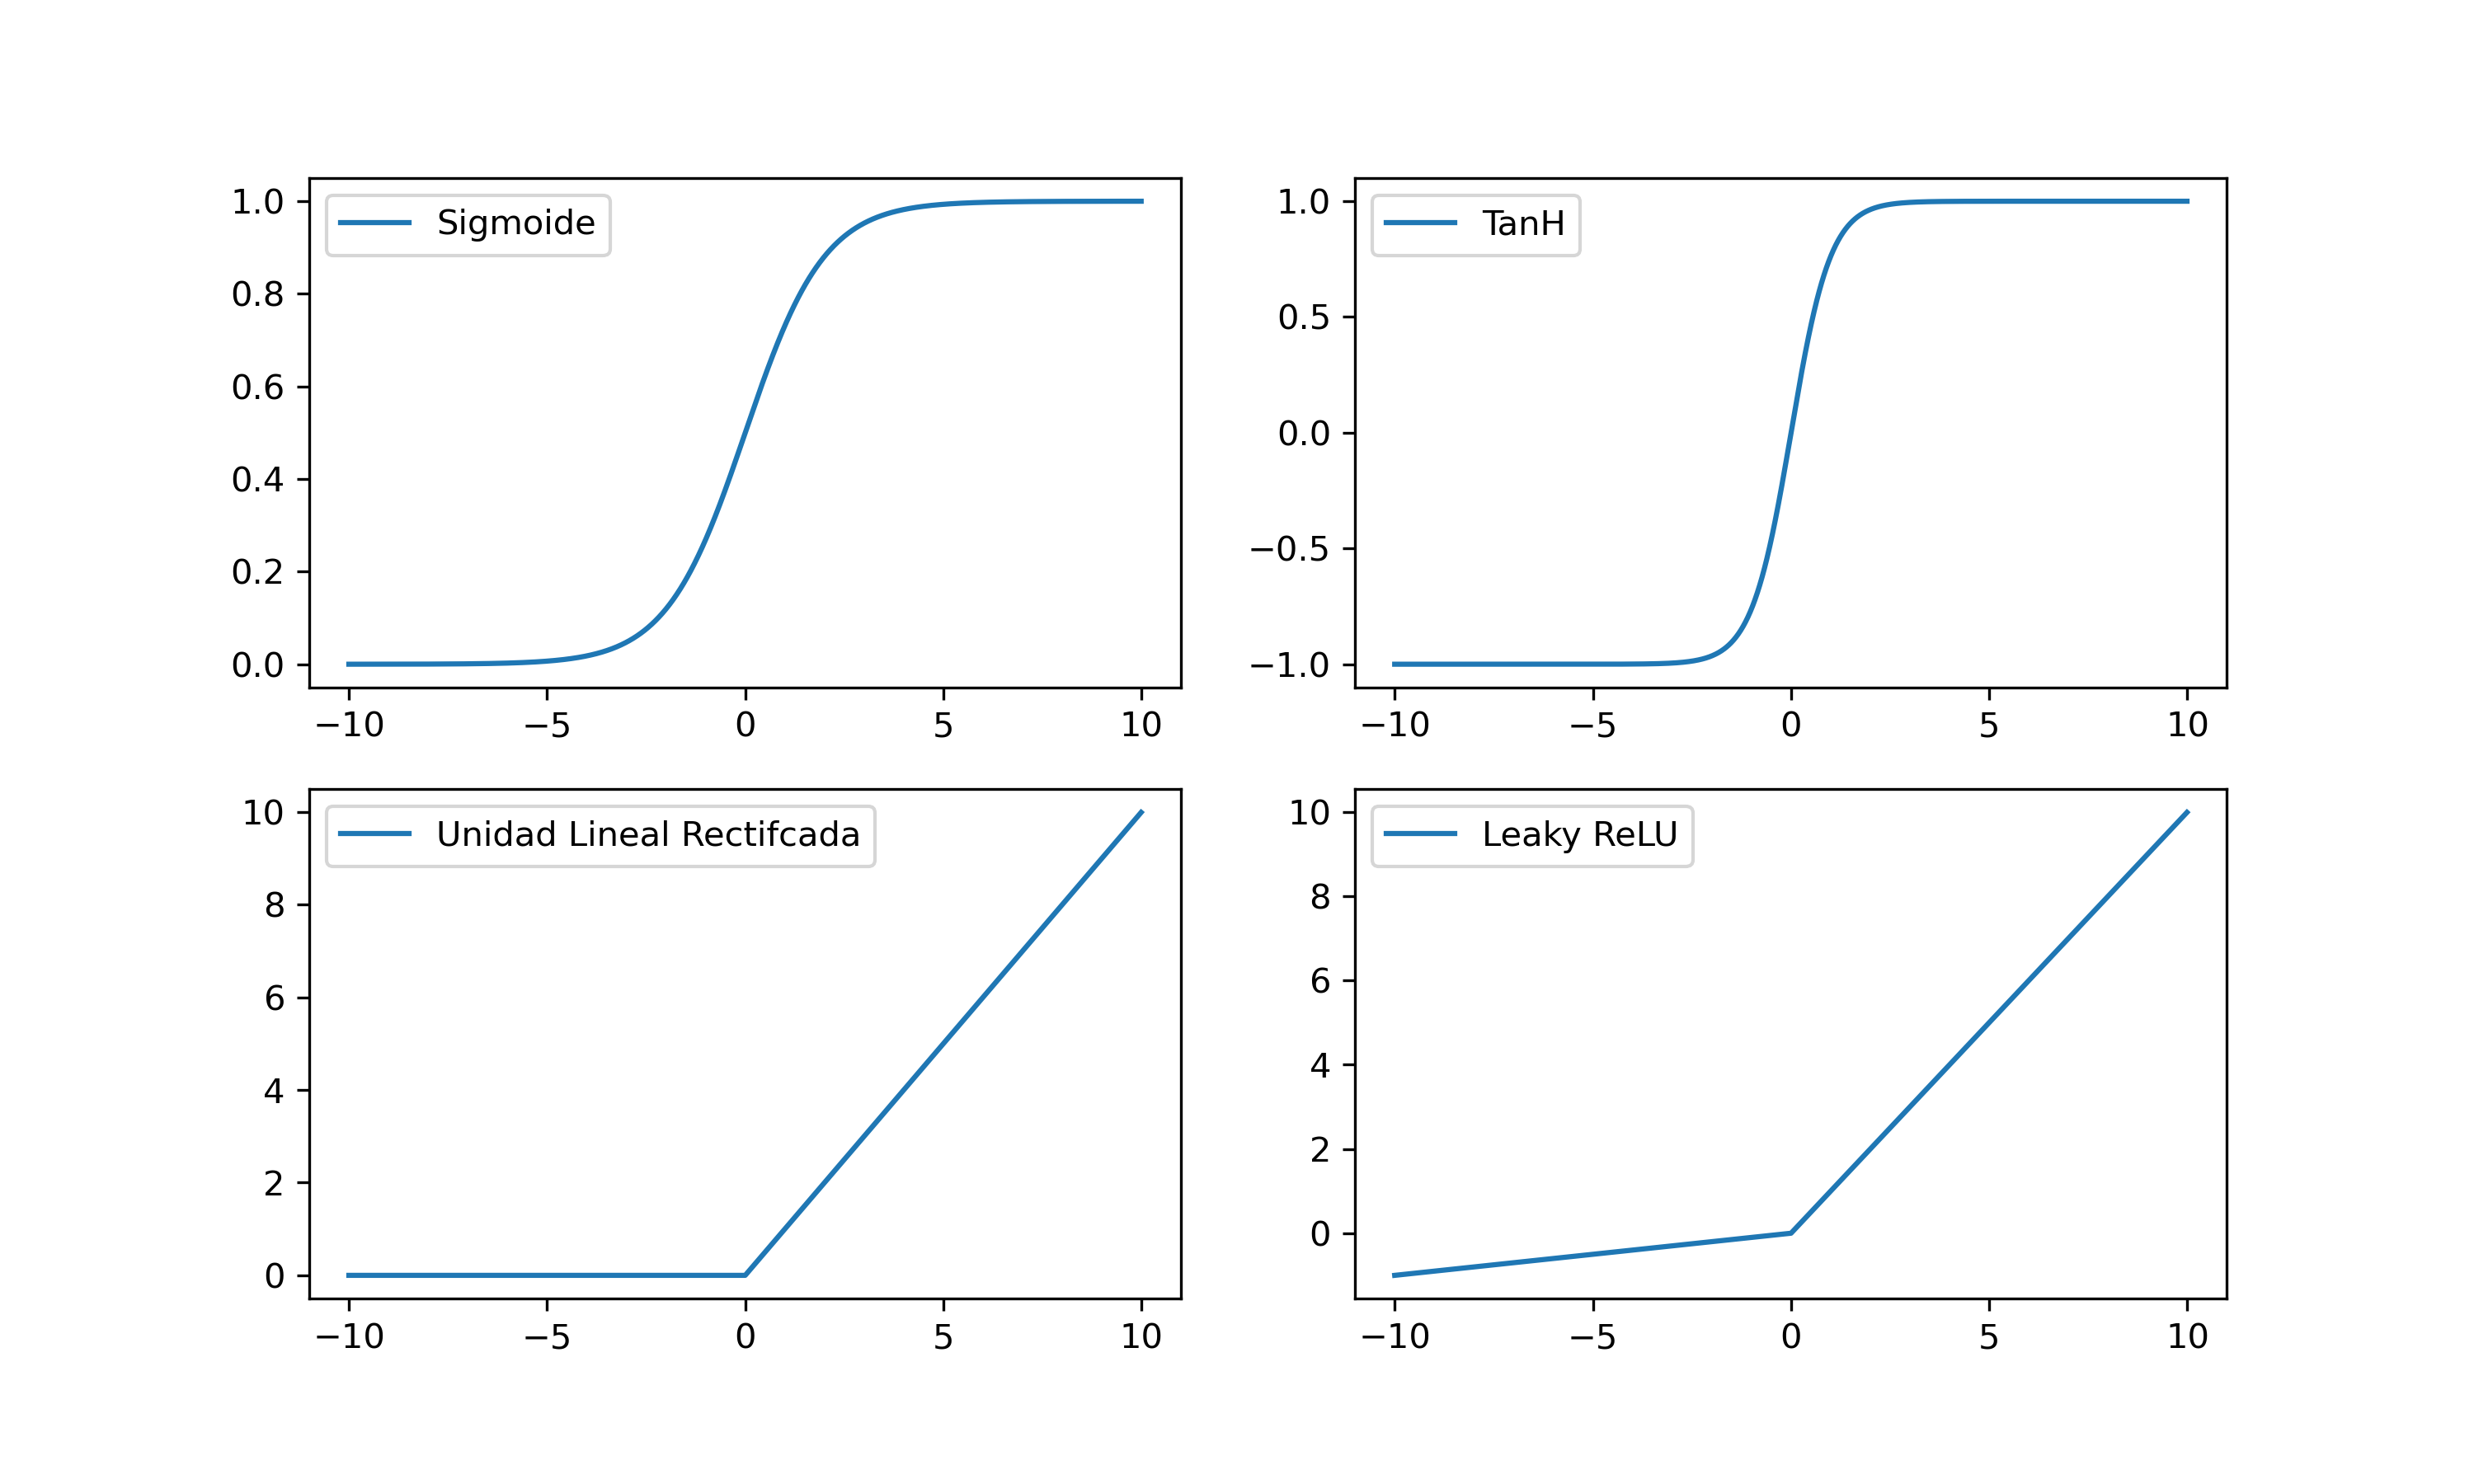
\includegraphics[width=\textwidth, keepaspectratio, height=7 cm]{images/funcionesdeactivacione.png}
            \caption{Funciones de activación}
            \label{fig:funciones de activacion}
        \end{figure}
\end{itemize}

El tipo de entrada que requiere las funciones de tensorflow/keras para el tipo
de modelo sequential, requieren un tipo de entrada numpy.array().
\begin{lstlisting}[language=Python, caption=Adecuación de los vectores de entrada usando numpy]
# 70% datos para entrenamiento, de mi dataset(datos Crudos)
## X = Matriz entrada (TA, DP) = (HR)
X_train = np.array(X_train)
## y = Salida (HR)
y_train = np.array(y_train)

# 30% datos para validacion, de mi dataset(datos Crudos)
## X = Matriz entrada (TA, DP)
X_test = np.array(X_test)
## y = Salida (HR)
y_test = np.array(y_test)

\end{lstlisting}

Finalmente para entrenar el modelo se utiliza la función model.fit(), contenida
en dentro de la clase sequential. utilizando como optimizador Adam, y metrica
de error(loss) Error Cuadrático medio.

A continuación se muestran algunos de los argumentos que requiere esta función.

\begin{itemize}\itemsep=-5px
    \item Entrada/salida(X\_train, y\_train): Estos argumentos representan en
        que variables se encuentran alojados los conjuntos que se utilizaran
        para entrenar los modelos. en este caso model2.
    \item Validation\_data: Sirve para representar la capacidad del modelo para
        estimar datos, siendo este un conjunto de datos externo a los datos de
        entrenamiento del modelo.
    \item Batch\_size: Representa la cantidad de muestras de los datos a cargar
        por etapa de entrenamiento.
\end{itemize}
\begin{lstlisting}[language=Python, caption=Funcion para entramiento]
model2.compile(optimizer=Adam(0.0001), loss='mse')
r = model2.fit(X_train, y_train,
              validation_data=(X_test,y_test),
              batch_size=16,
              epochs=800)
\end{lstlisting}
\subsection{Análisis de resultados para distintos casos y arquitecturas}

Métricas de evaluación usadas para la revisión de los modelos, a continuación
se describen algunas de las medidas mas comunes. 

\textbf{Simbolos}:  
\begin{itemize}
    \item{\textbf{$y_i$}: Resultado real esperado}
    \item{\textbf{$\hat{y}_i$}: Predicción del modelo}
    \item{\textbf{$n$}: Tamaño de la muestra}
\end{itemize}
Error absoluto medio (MAE): Es la media del error absoluto 
\begin{equation*}
    \frac 1n\sum_{i=1}^n|y_i-\hat{y}_i|
\end{equation*}

Error Cuadrático medio (MSE) Este es el promedio de los errores cuadráticos
medios

\begin{equation*}
    \frac 1n\sum_{i=1}^n(y_i-\hat{y}_i)^2
\end{equation*}
\begin{itemize}
    \item Ventajas 

        Útil si se tienen valores inesperados, que nos deberian interesar, muy
        alto o bajo valor que debemos prestar atencion.

    \item Desventajas 

        Si hacemos un predición muy mala, la cuadratura empeorara aun mas el
        error y puede sesgar la metrica para sobreestimar la maldad del modelo.
        Este es un compartamiento particularmente problemático si tenemos datos
        ruidosos. 

\end{itemize}

Raíz del error cuadrático medio (RMSE) Es la raíz cuadrado de la media del
error de cuadrados:
\begin{equation*}
    \sqrt{\frac 1n\sum_{i=1}^n(y_i-\hat{y}_i)^2}
\end{equation*}

Características generales de los errores. 

\textbf{MAE} Este es el mas sencillo de entender, siendo este el promedio el
error en la muestra. 

\textbf{MSE} Este tiene características similares al MAE, sin embargo este
tiende a disminuir los errores largos, que terminan siendo inútiles en
aplicaciones reales. 

\textbf{RMSE} Este es útil dado que los valores se pueden interpretar en
función de la salida.

Todos estos sirven para entrenar a una red neuronal, serian las funciones de
perdida que buscamos minimizar, haciendo uso de los distintos algoritmos de
optimización, en este caso estamos haciendo uso en la mayor parte del
optimizador Adam.

Para calcular esto errores se tiene las siguiente funciones en python. 
\begin{lstlisting}[language=Python, label=f_eval, caption= definicion de
funciones de evaluacion utilizando sklearn como herramienta base]
#Librerias
from sklearn import metrics
from sklearn.model_selection import cross_val_score
#Funcion de evaluacion para imprimir en la consola.
def print_evaluate(true, predicted):  
    mae = metrics.mean_absolute_error(true, predicted)
    mse = metrics.mean_squared_error(true, predicted)
    rmse = np.sqrt(metrics.mean_squared_error(true, predicted))
    r2_square = metrics.r2_score(true, predicted)
    print('MAE:', mae)
    print('MSE:', mse)
    print('RMSE:', rmse)
    print('R2 Square', r2_square)
    print('__________________________________')
'''
Funcion de evaluacion que devuelve variables, para ser usadas en alguna otra
funcion.ej. para crear una data frame en pandas con las metricas de evaluacion. 
'''
def evaluate(true, predicted):
    mae = metrics.mean_absolute_error(true, predicted)
    mse = metrics.mean_squared_error(true, predicted)
    rmse = np.sqrt(metrics.mean_squared_error(true, predicted))
    r2_square = metrics.r2_score(true, predicted)
    return mae, mse, rmse, r2_square
\end{lstlisting}

Haciendo uso de las funciones del código \ref{f_eval}, se evalúan los modelos
ya entrenados. Con dos  salida posibles por la salida estándar en tipo crudo, y
en formato de salida de pandas.

\begin{lstlisting}[language=Python, caption=Funciones  utilizadas en la
evaluación de los modelos]
# stdout
test_pred = model2.predict(X_test)
train_pred = model2.predict(X_train)
print('Test set evaluation:\n_____________________________________')
print_evaluate(y_test, test_pred)
print('Train set evaluation:\n_____________________________________')
print_evaluate(y_train, train_pred)
# dataframe de resultados
results_df = pd.DataFrame(data=[["NN para UAS 2019-2020", *evaluate(y_test, test_pred)]],columns=['Model', 'MAE', 'MSE', 'RMSE', 'R2 Square'])
results_df
\end{lstlisting}
\begin{table}[H]
    \centering
    \begin{tabular}{|p{5cm}|p{2cm}|p{2cm}|p{2cm}|p{2cm}|}\hline
        Modelo & MAE	& MSE	&RMSE	&R2 Square\\\hline
        NN para UAS 2019-2020 & 5.680064 & 43.625018 & 6.604924	& -1.575113\\
        \hline
    \end{tabular}
    \caption{Salida(tipo dataframe) para el modelo entrenado para los datos uas
    2019-2020}
    \label{model1}
\end{table}

El cuadro \ref{model1}, corresponde a una arquitectura  de capa interconectada
completamente o también llamada de capas densas:
[2,dropout(0.2),64,dropout(0.2),128,dropout(0.2),32,dropout(0.2),1]; usando
como algoritmo de optimización Adam, y un tamaño de batch = 16, con un total de
800 épocas(veces que se repite el proceso de entrenamiento).

Análisis de los resultados usando un gráfico de dispersión, de los valores
reales contra los valores predichos por dichos modelos. 

\begin{figure}[H]
    \centering
    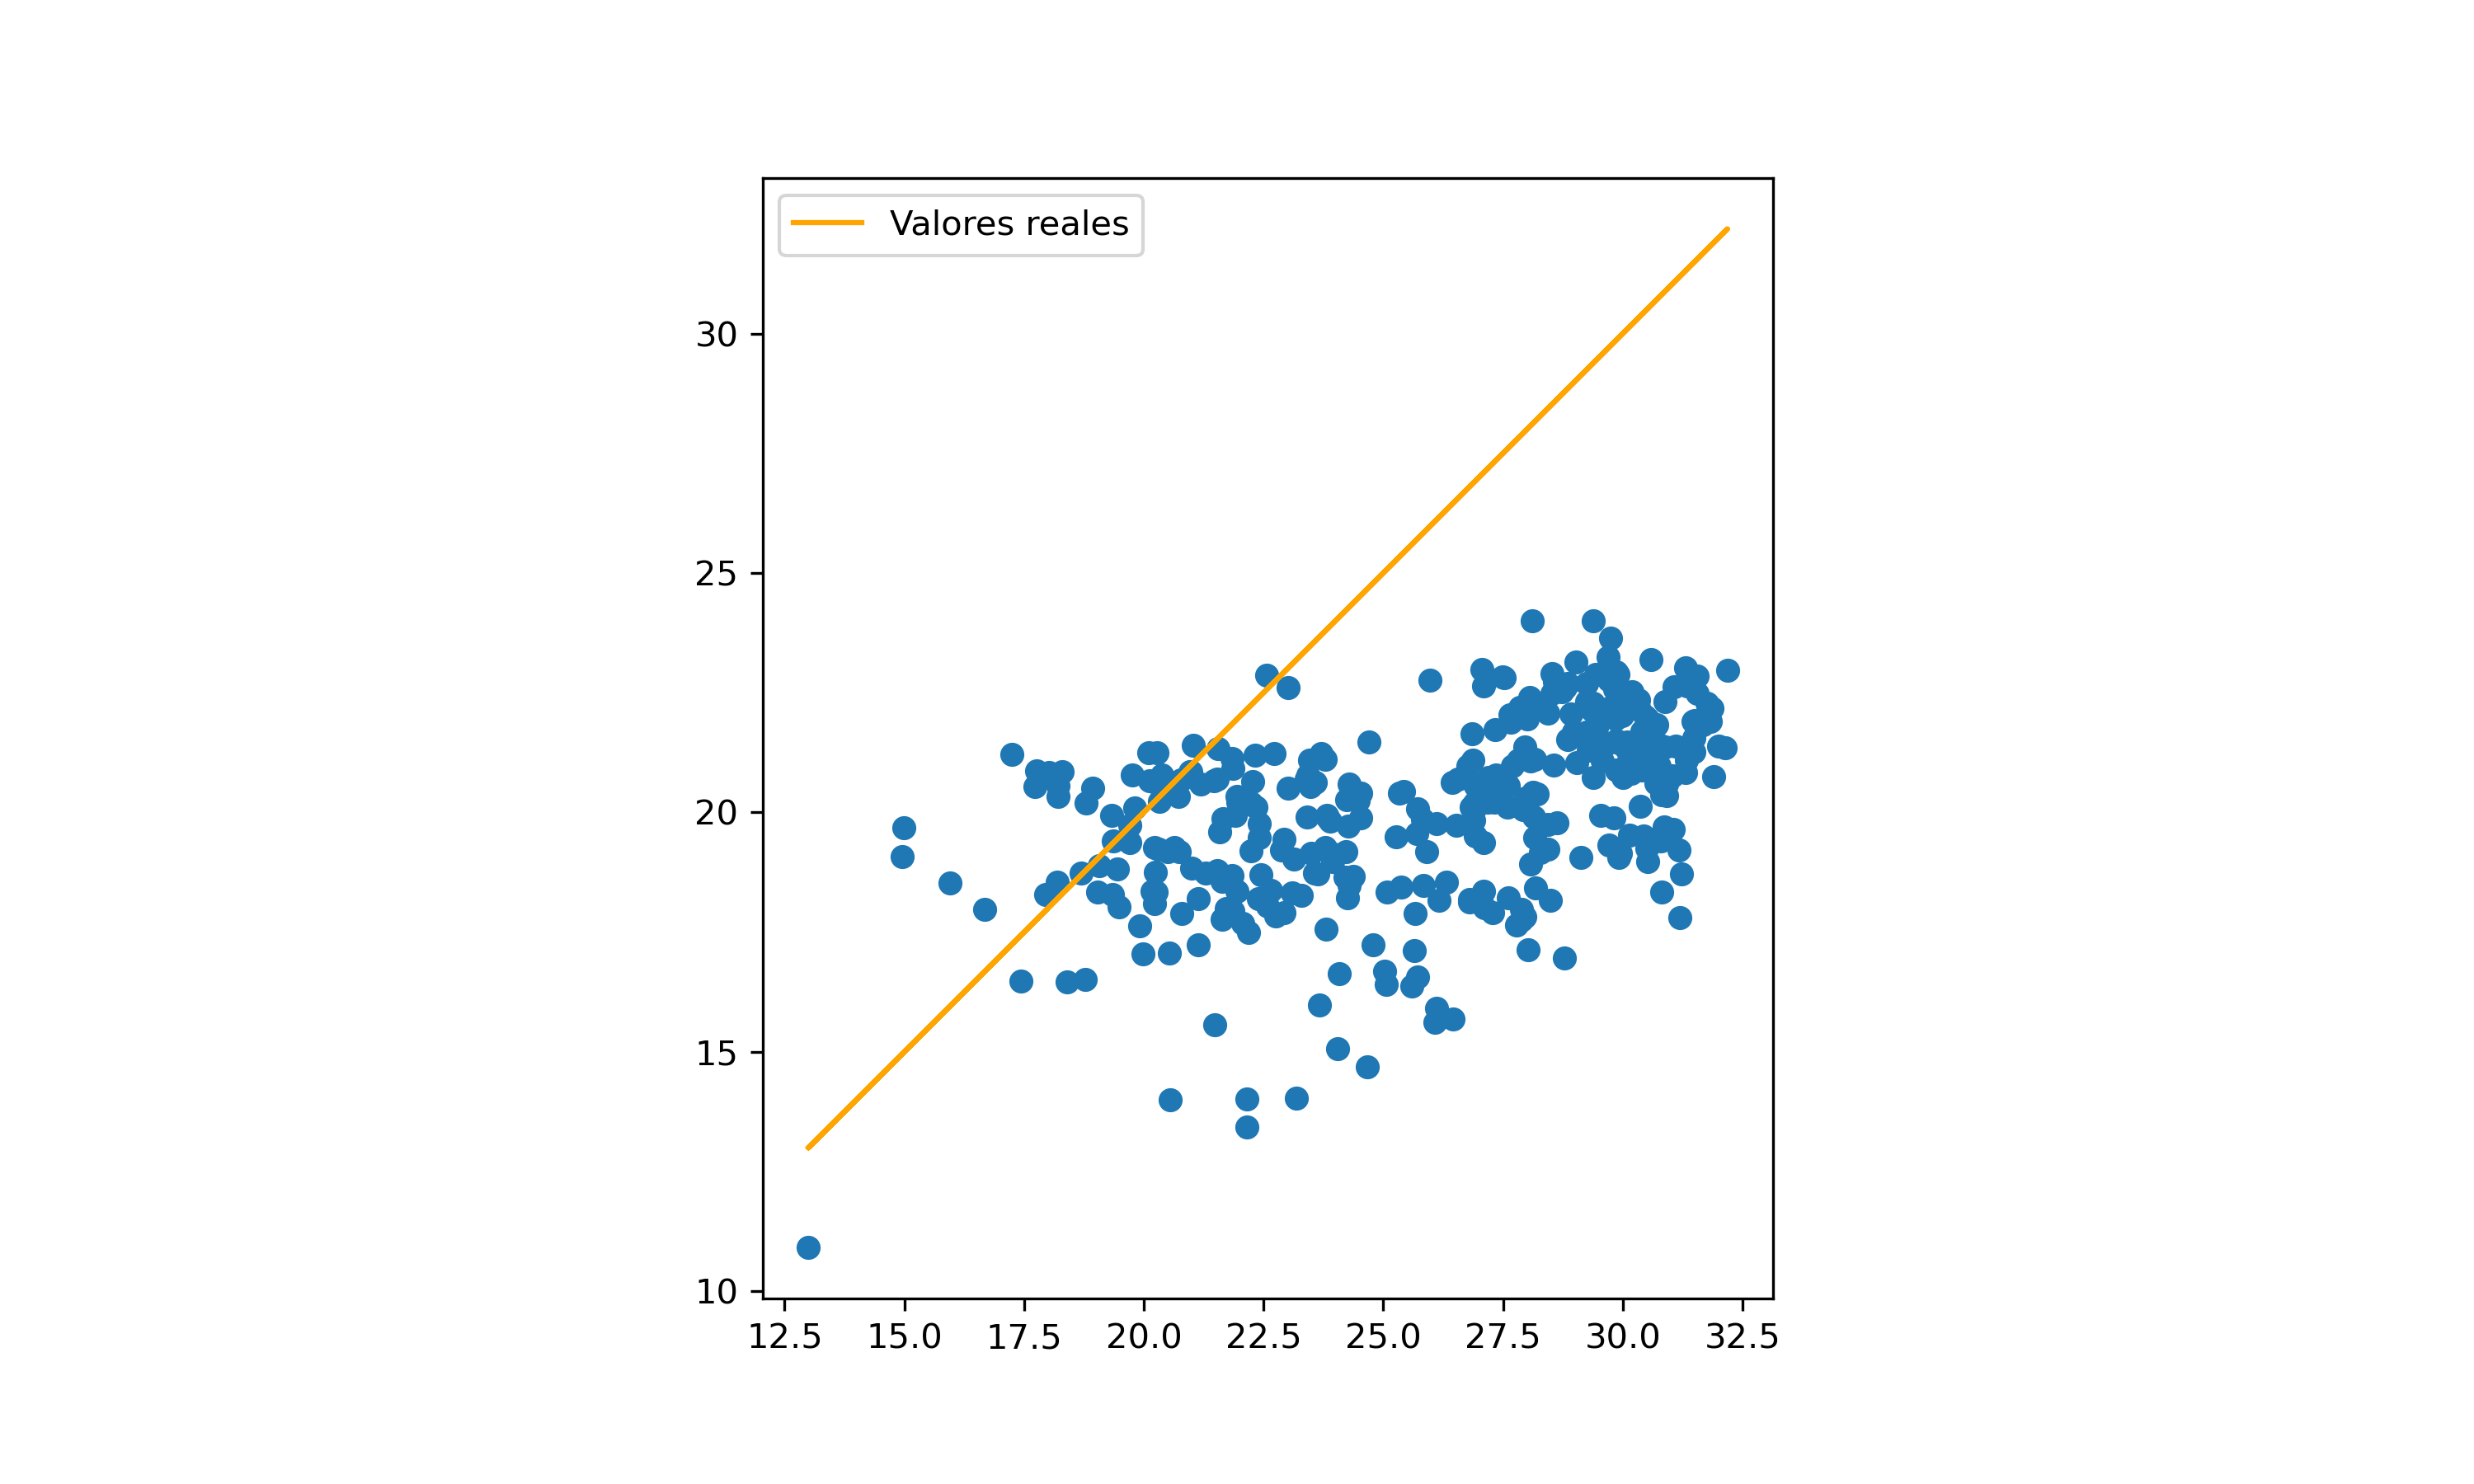
\includegraphics[width=\textwidth, keepaspectratio,
    height=7cm]{images/resultados-modelo1-dispersion.png}
    \caption{Gráfico de dispersión del modelo "NN para UAS 2019-2020"}
    \label{fig:dispersion-resultados-uas}
\end{figure}


\begin{lstlisting}[language=Python, caption=]

\end{lstlisting}

\begin{lstlisting}[language=Python, caption=]

\end{lstlisting}
\begin{lstlisting}[language=Python, caption=]

\end{lstlisting}
\begin{lstlisting}[language=Python, caption=]

\end{lstlisting}
\begin{lstlisting}[language=Python, caption=]

\end{lstlisting}
\begin{lstlisting}[language=Python, caption=]

\end{lstlisting}
